\documentclass[12pt, twoside, a4paper]{report}
\usepackage{amsmath}
\usepackage{ragged2e}
\usepackage{fancyhdr}
\usepackage{graphicx}
\usepackage{float}
\usepackage{hyperref}

\title{CS2810 - Group Report}
\author{Marcus Messer, Toby Such, Roger Milroy, Andrew Nicolalde,\\
Jonathan Lewin, Robin Chabouk, Johan Rehman}
\date{\today}

\begin{document}
\maketitle
\pagestyle{fancy}
\fancyhf{}
\lhead{CS2810 - Group Report}
\rfoot{Page \thepage}

\chapter*{Description Of Components}
\section*{Views}
See \textit{\nameref{sec:static}} for links to the Java Script Documentation.
\subsection*{Customer}
\subsubsection*{Start Order Page}

\subsubsection*{Menu Page}
Once the customer has clicked Start Order, they will be brought to the Menu Page. The customer can now pick which items they want to order by searching through four different categories. See \textit{Figure \ref{fig:menuClosed}} and \textit{Figure \ref{fig:menuOpen}}.

\begin{figure}[H]
  \centering
  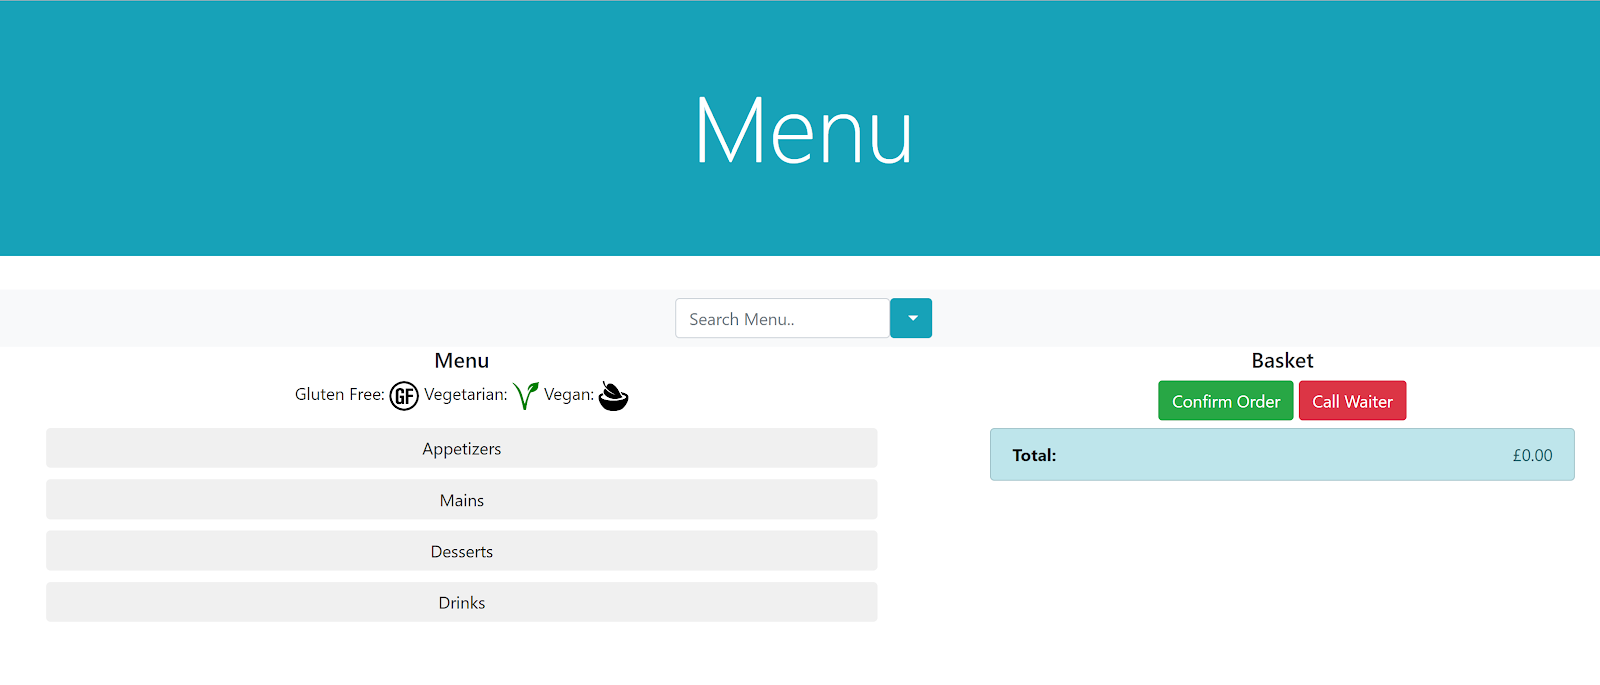
\includegraphics[width=10cm]{MenuClosed.png}
  \caption{The Menu Page with Closed Categories}
  \label{fig:menuClosed}
\end{figure}

\begin{figure}[H]
  \centering
  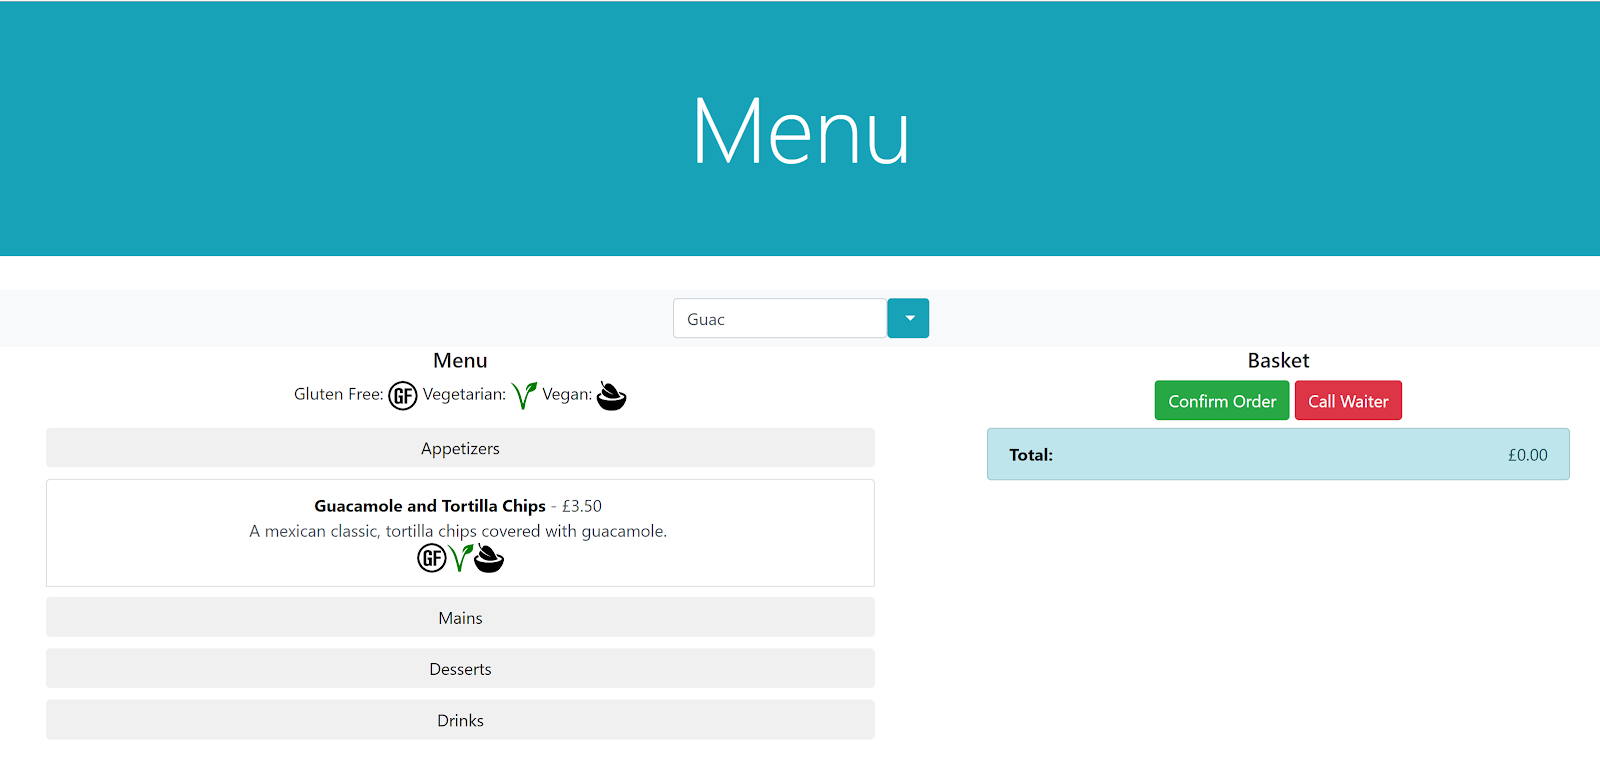
\includegraphics[width=10cm]{MenuOpen.png}
  \caption{The Menu Page with Open Categories}
  \label{fig:menuOpen}
\end{figure}

A customer can also search for an item, filtering by a specific category (vegan/vegetarian/gluten free) which will only display items that meet the category criteria. See \textit{Figure \ref{fig:menuFilter}}.

\begin{figure}[H]
  \centering
  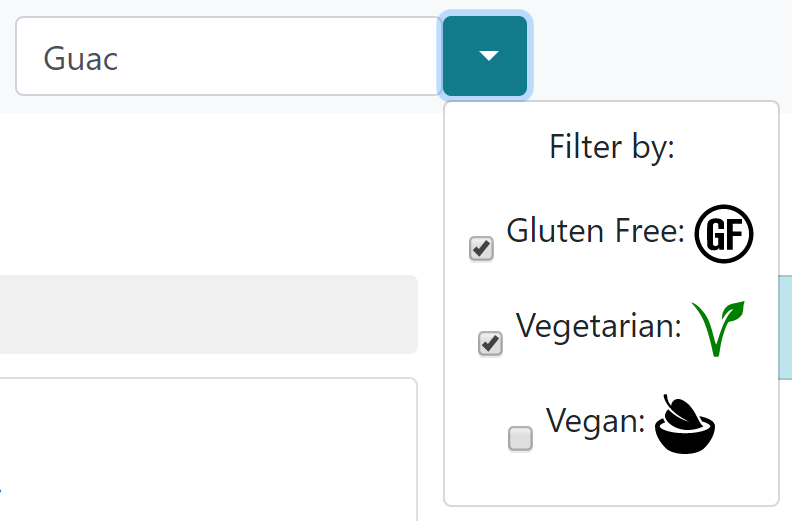
\includegraphics[width=5cm]{MenuFilter.png}
  \caption{The Menu Filtering Section}
  \label{fig:menuFilter}
\end{figure}

Once the customer clicks on the menu item they want to order, an item summary will pop up and will display more information such as the Price and the description of the item.
They can also add specific instructions that will then be seen by the chefs that cook the meal.
When the customer clicks the ‘Add to Order’ button, the order is added to the list.
See \textit{Figure \ref{fig:menuItem}}.

\begin{figure}[H]
  \centering
  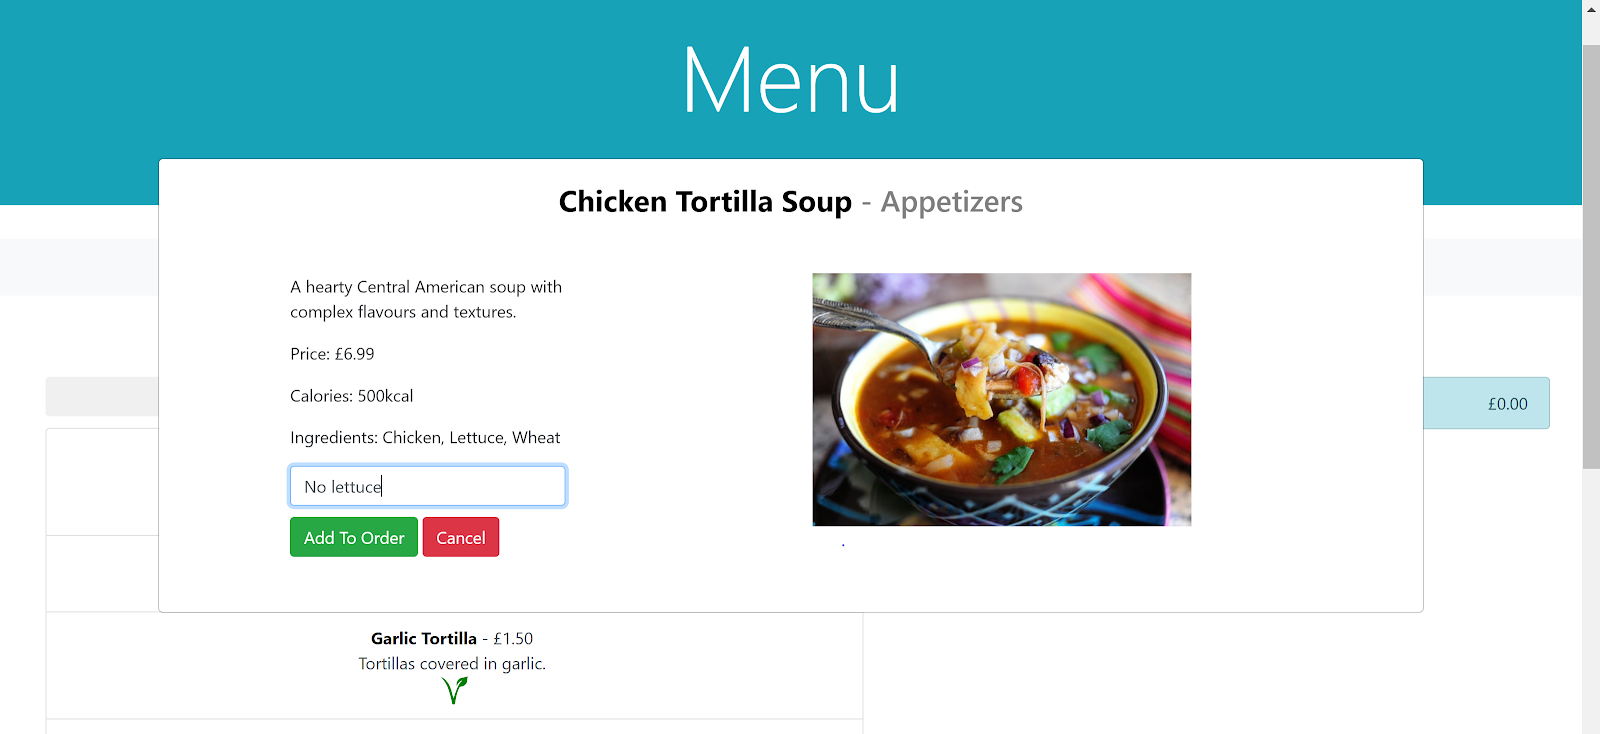
\includegraphics[width=10cm]{MenuItem.png}
  \caption{The Menu Item Modal}
  \label{fig:menuItem}
\end{figure}

The menu items that the customer has added to the order is then displayed under the basket order list. This list will show the items that have been added, their individual price and the total price. Once the customer is happy that they have all the items they want to order, they will click ‘Confirm Order’ to send the list to the basket page. See \textit{Figure \ref{fig:menuOrder}}.

\begin{figure}[H]
  \centering
  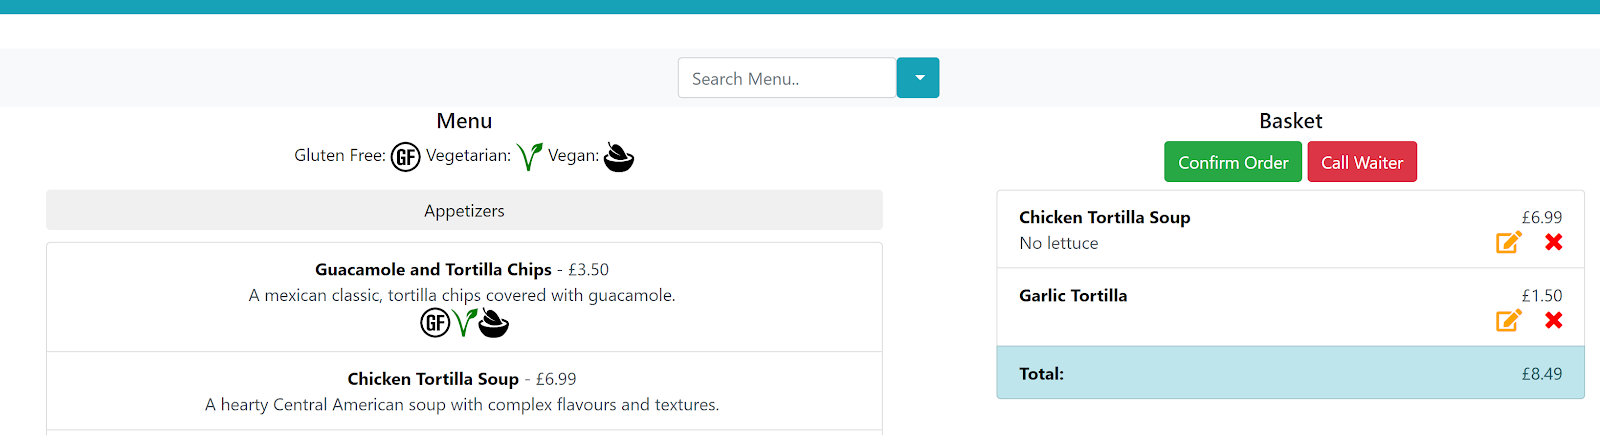
\includegraphics[width=10cm]{MenuOrder.png}
  \caption{The Menu Page with an Order}
  \label{fig:menuOrder}
\end{figure}

\subsubsection*{Basket Page} 

See \textit{Figure \ref{fig:basket}}.

This is the page the customer is taken to once they have selected and confirmed what they want to order. Customers can add to the same order by navigating to the basket page via the link in the top right of the page, or can start a new order by navigating to the home page.

Each order has an order number, shows the status of the order (along with a little symbol that reflects this) and the price for that order. Orders contain a table with all the items in that order. The table includes the name of each item, a short description, any instructions that were added and the price. If more than one of the same item is added to the order, it is shown by a repetition of the item in the order table.

At the bottom of the accordion element the total price is displayed for all orders so that customers have an up to date idea of how much their meal is costing them. The call waiter button simply notifies a waiter that the particular table needs assistance and confirms with the customer that this has been done via a modal. There is also a back to menu button next to call waiter for convenience.

This view gives the customer a good idea of what is going on with their orders and allows them to plan what else they may want to get accordingly.

\begin{figure}[H]
  \centering
  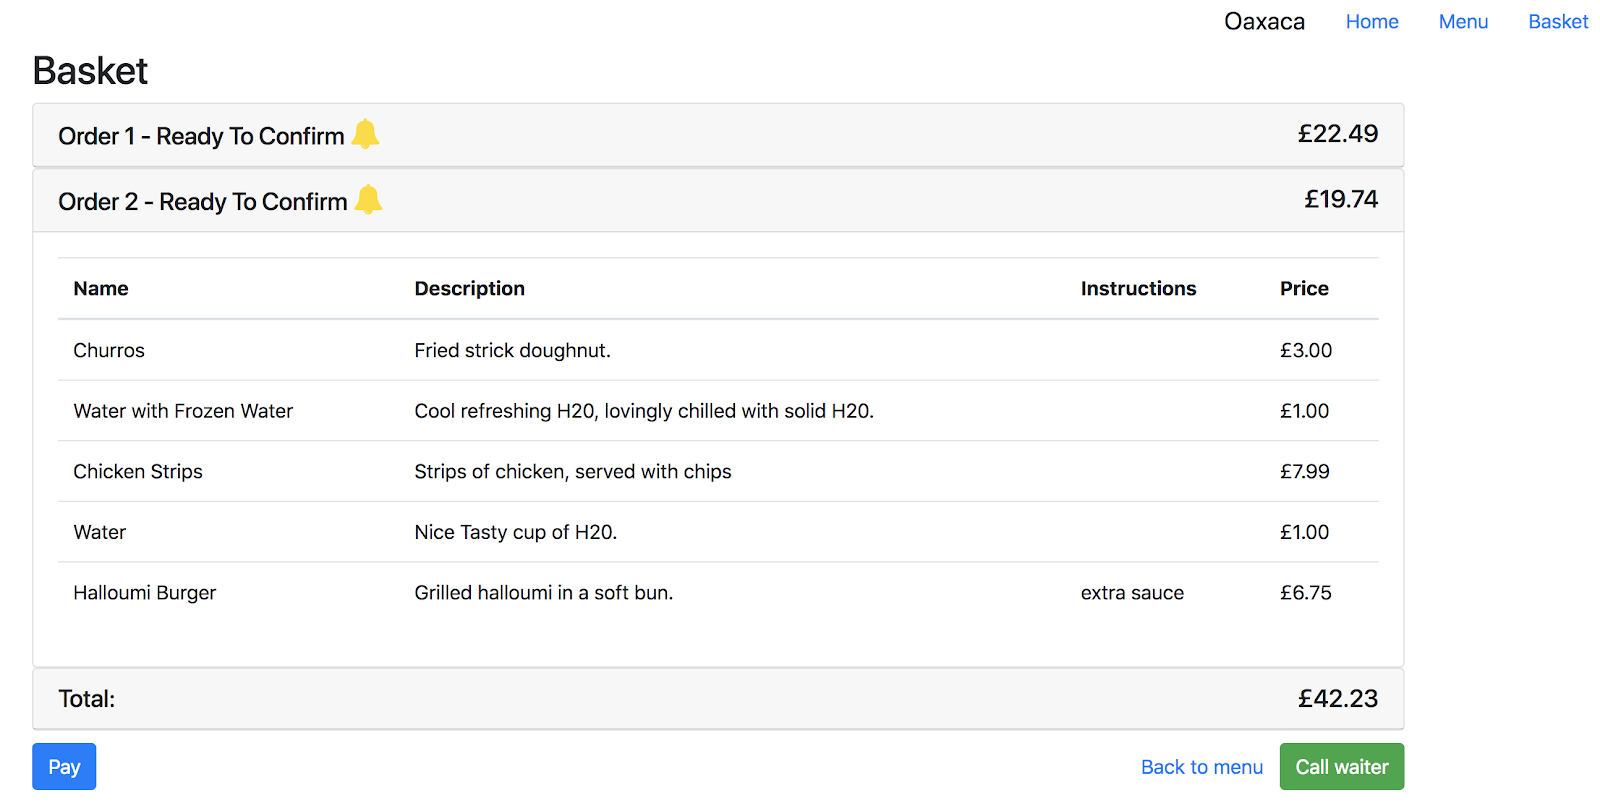
\includegraphics[width=10cm]{basket.png}
  \caption{The Customer's Basket Page}
  \label{fig:basket}
\end{figure}

\subsubsection*{Payment}
This is the payment form, see \textit{Figure \ref{fig:pay}}. It forms a part of the Basket page and is made visible when the pay button is pressed.
On this page, the customer enters several details. Their email address is used to send the customer an email receipt, and their card details are used to debit their account.
The user enters these details and then clicks the “Pay” button, which also displays the total for the Transaction.
Upon successful payment, the customer will be redirected to the start order page and they will be free to leave.

\begin{figure}[H]
  \centering
  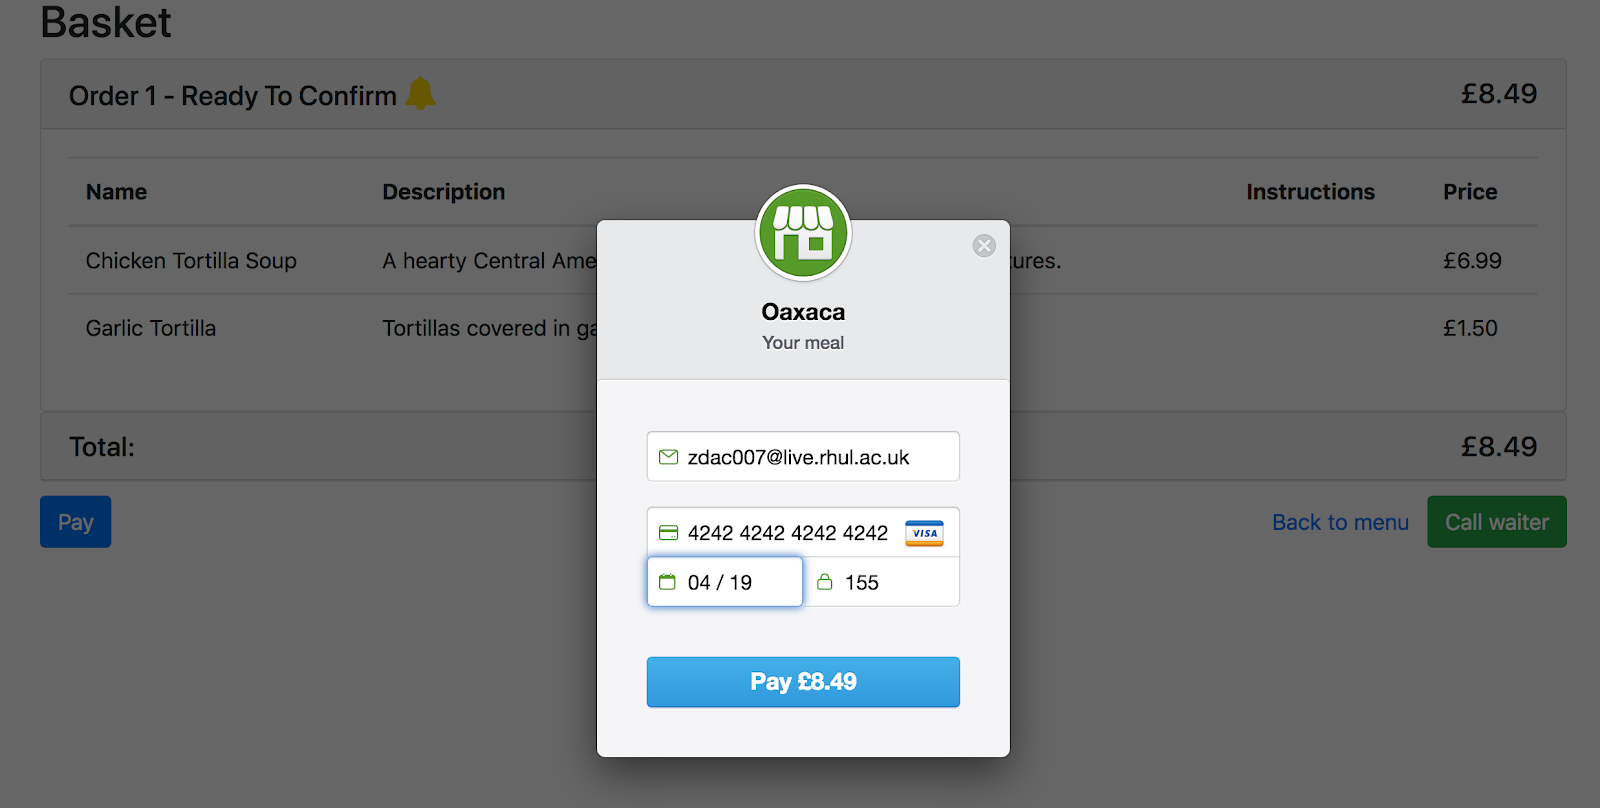
\includegraphics[width=10cm]{Payment.png}
  \caption{The Customer's Payment Form}
  \label{fig:pay}
\end{figure}

\subsection*{Waiter}
\subsubsection*{Orders Page}

\subsubsection*{Edit Order View}

\subsection*{Kitchen}

\subsection*{Manager}
\subsubsection*{Manager Home Page}

\subsubsection*{Edit Menu Page}

\subsubsection*{Assign Tables Page}

\subsubsection*{Employee Page}

\section*{Server}
The server is responsible for providing communication and authentication between the user interface and the database.
We use Spark to handle the communication between the front end and the server itself. We have created numerous classes for the purpose, more detail is provided in \textit{\nameref{sec:endpoints}}.
Also handled by the server is the communication and the creation of the database, we use the Hibernate ORM and JPA to create and communicate to the PostgreSQL database. More detail on how this is done is provided in \textit{\nameref{sec:database}}.

\section*{Database}

We have a database with 19 related tables, see \textit{Figure \ref{fig:data}}. 

The database stores everything including the staff, the menu and the customers orders. 
It also stores the logged in sessions and the data needed for push notifications.
The database was designed to allow the user to start multiple orders and store them onto a transaction that allows the users to pay for all there orders in one go.

\begin{figure}[H]
  \centering
  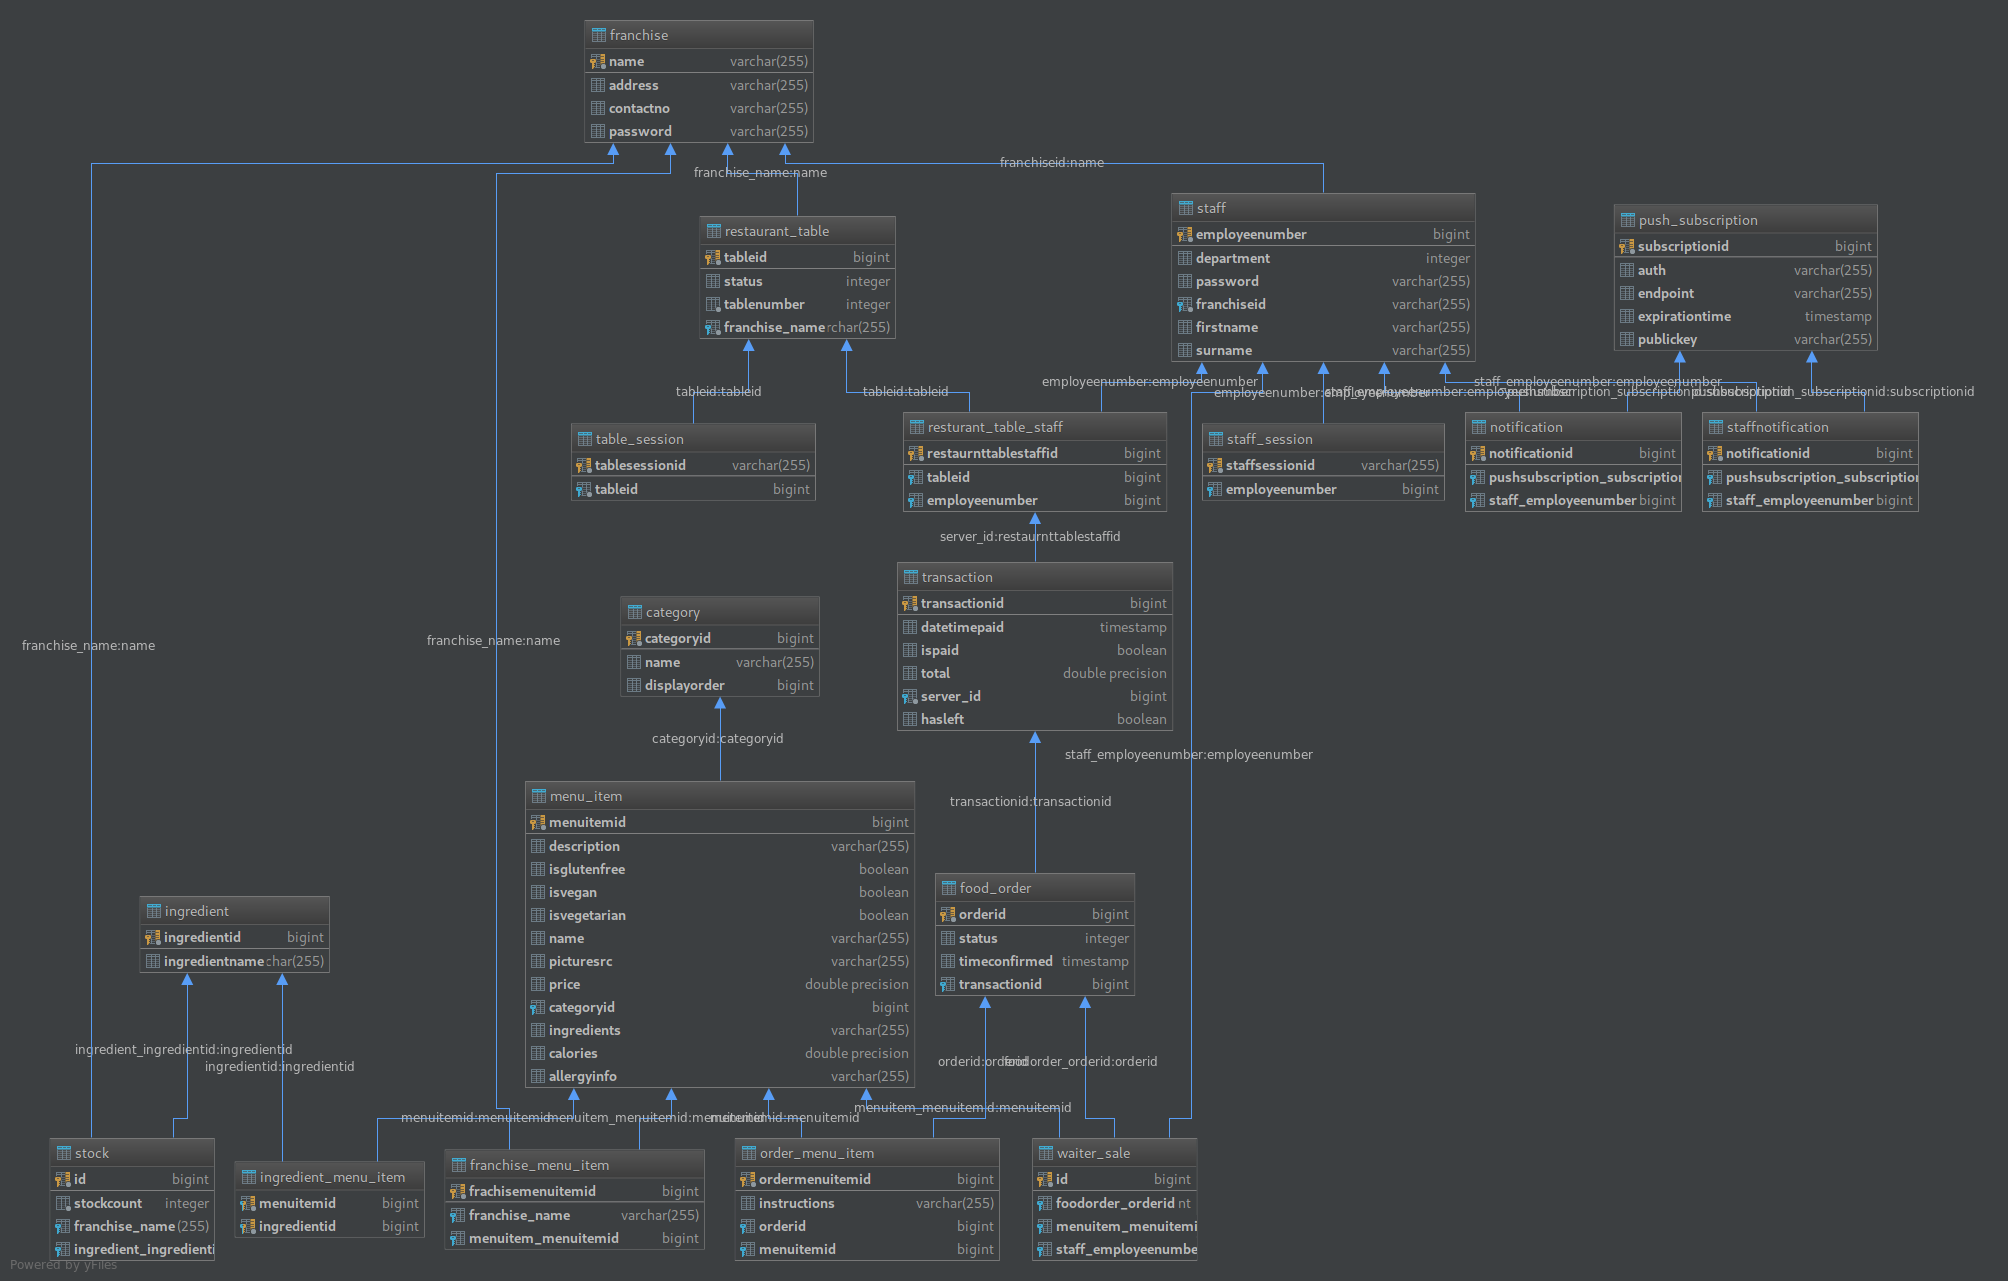
\includegraphics[width=15cm]{database.png}
  \caption{Generated by DataGrip}
  \label{fig:data}
\end{figure}

\chapter*{Description Of Packages}
\section*{Database}\label{sec:database}
\subsection*{Implemented Components}
This package implements the following components:
\begin{itemize}
  \item A fully relational database in hopefully third normal form. All created with Hibernate ORM.
  \item A Database Manager Singleton for easy access to creating JPA Entity Managers, without the need of creating more than one factory.
\end{itemize}
\subsection*{Functionality}
For details on the functionality see \textit{\href{run:../JavaDoc/database/package-summary.html}{the Database Package overview}} and \textit{\href{run:../JavaDoc/database/tables/package-summary.html}{the Table Package overview}}.

\section*{Endpoints}\label{sec:endpoints}
\subsection*{Implemented Components}
This package contains classes that link the front end to the database.
\begin{itemize}
  \item Authentication classes to authenticate a users login to stop unauthorized access.
  \item Ingredient classes to provide end points that interact with the ingredient table in the database.
  \item Manger classes to provide the end points necessary to create the implemented manager user stories.
  \item Menu classes to provide the end points needed to load and edit the menu.
  \item Notification classes that provide our push notification service, including auto updating the web pages.
  \item Order classes to provide the ability to create, view and edits for both the customer view and the waiter view.
  \item Payment classes to provide the Stripe functionality so they customers can pay by card.
  \item Table classes to get the list of table, change there status and change which waiters are assigned to which table.
  \item Transaction classes to allow the front end to get details on the current transaction.
\end{itemize}

\subsection*{Functionality}
See the following Java Doc overviews for more details:
\begin{itemize}
  \item \textit{\href{run:../JavaDoc/endpoints/authentication/package-summary.html}{Authentication}}
  \item \textit{\href{run:../JavaDoc/endpoints/ingredient/package-summary.html}{Ingredients}}
  \item \textit{\href{run:../JavaDoc/endpoints/manager/package-summary.html}{Manger}}
  \item \textit{\href{run:../JavaDoc/endpoints/menu/package-summary.html}{Menu}}
  \item \textit{\href{run:../JavaDoc/endpoints/notification/package-summary.html}{Notification}}
  \item \textit{\href{run:../JavaDoc/endpoints/order/package-summary.html}{Order}}
  \item \textit{\href{run:../JavaDoc/endpoints/payment/package-summary.html}{Payment}}
  \item \textit{\href{run:../JavaDoc/endpoints/tables/package-summary.html}{Tables}}
  \item \textit{\href{run:../JavaDoc/endpoints/transaction/package-summary.html}{Transaction}}
\end{itemize}

\section*{Static}\label{sec:static}
\subsection*{Implemented Components}
\subsection*{Functionality}

\section*{Utility}\label{sec:util}
\subsection*{Implemented Components}
\subsection*{Functionality}

\chapter*{User Stories}
\section*{Fully Completed}
These are the completed user stories.
\subsection*{Customer Stories}
\begin{itemize}
  \item Electronic Payment
  \item View Menu
  \item Ordering
  \item Menu Filtering
  \item Calling The Waiter
  \item Allergies And Calories
  \item Food Pictures
  \item Order Tracking
  \item Intuitive Ordering
\end{itemize}

\subsection*{Waiter Stories}
\begin{itemize}
  \item Notification For Delivery
  \item Cancel Order
  \item Order Times
  \item Payment Information
  \item Order Confirmation
  \item Table Assignment
  \item Mark Order as Delivered
  \item Client Needs Help
  \item Add Extra Sales
  \item Change Status Of An Order
\end{itemize}

\subsection*{Kitchen Stories}
\begin{itemize}
  \item Notify Waiters
  \item Confirmed Customer Order
  \item Order Times
\end{itemize}

\subsection*{Manager Stories}
\begin{itemize}
  \item Assign Tables
  \item Set Prices
\end{itemize}

\section*{Nearly Completed}
These stores are worthy of a mention as they are very nearly finished.

\subsection*{Manager Stories}
\begin{itemize}
  \item Adjust Menu:
    The only feature left uncompleted is uploading an image to the new menu item or when editing a menu item.
  \item Add Staff:
    The only feature left is the ability to reset a users password.
\end{itemize}

\chapter*{Statement of Relative Contribution}
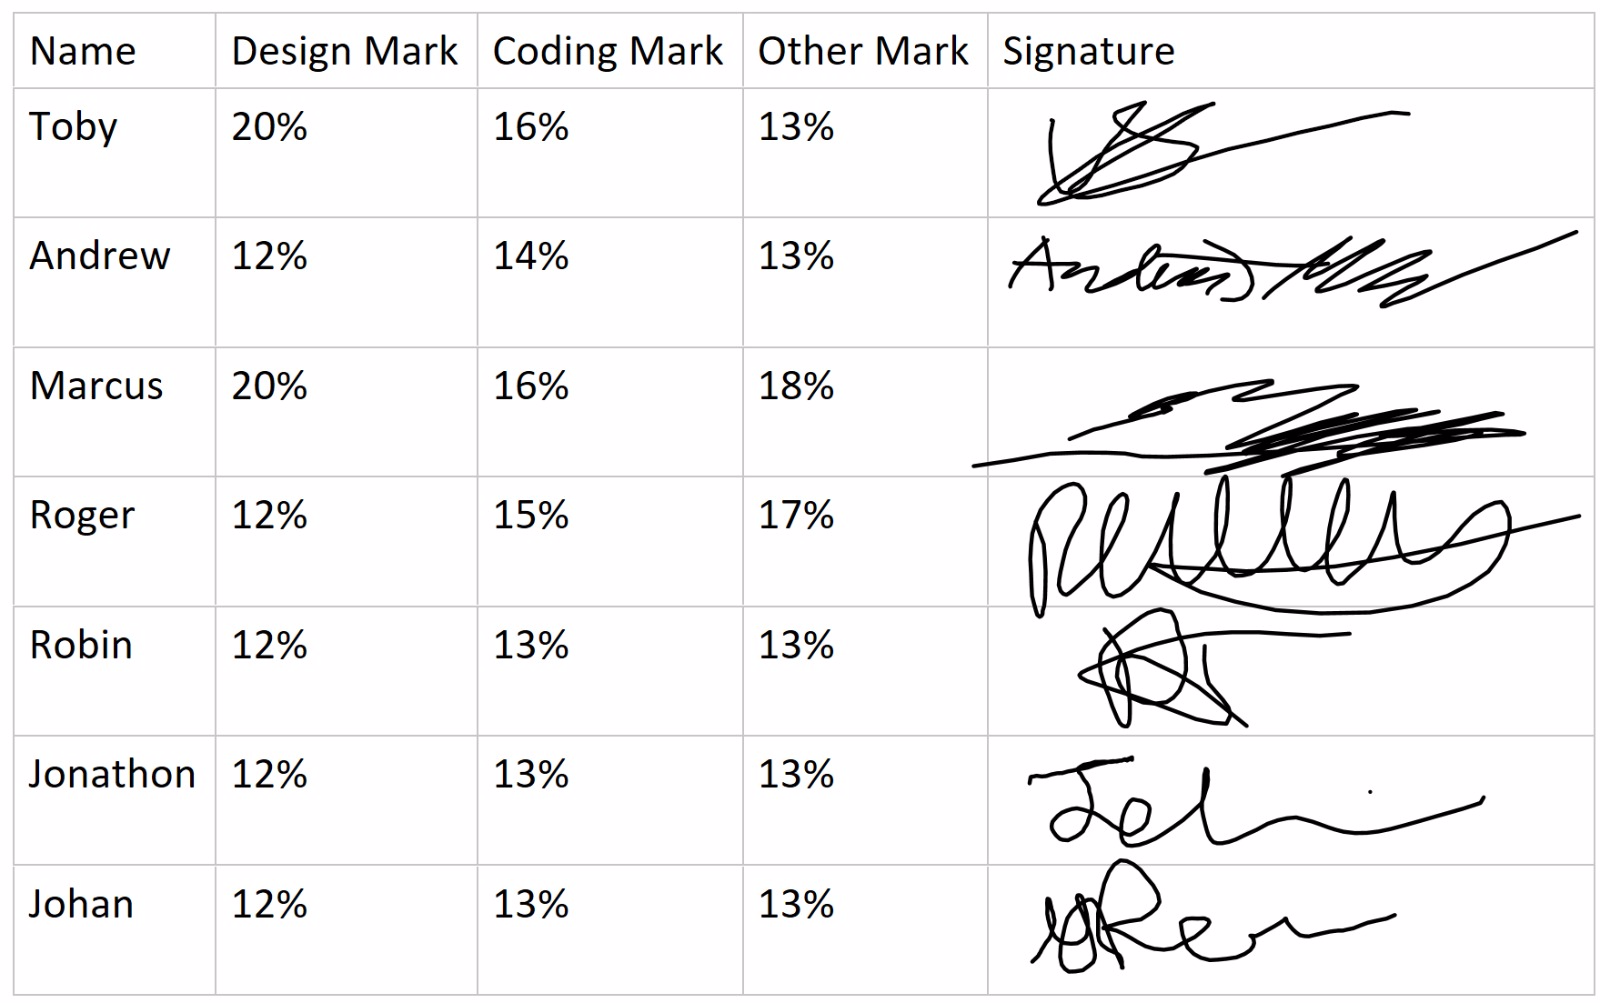
\includegraphics[width=15cm]{StateOfCont.png}

\end{document}
